\documentclass[conference]{IEEEtran}
\usepackage[spanish,es-tabla,es-noshorthands]{babel}
\usepackage{fontspec}
\setmainfont{Times New Roman}
\usepackage{amsmath}
\usepackage{graphicx}
\usepackage{booktabs}
\usepackage{array}
% \captionof, como en el paquete capt-of: un título de tabla fuera de un flotante.
\makeatletter\newcommand\captionof[1]{\def\@captype{#1}\caption}\makeatother
\usepackage{xurl}
\usepackage[hidelinks]{hyperref}
\hypersetup{pdftitle={Robo denunciado por pasajero en el metro de la CDMX: qué estaciones cambian de lugar al medir por millón de entradas}, pdfauthor={Sebastián Córdoba}}
\graphicspath{{../figuras/metro/}}
\renewcommand{\IEEEkeywordsname}{Palabras clave}
\newcommand{\pme}{por millón de entradas}
\newcolumntype{L}[1]{>{\raggedright\arraybackslash}p{#1}}
% Párrafos sin sangría, separados por un poco de espacio vertical.
\setlength{\parindent}{0pt}
\setlength{\parskip}{0.4\baselineskip}
% Menos aire entre flotantes y texto (IEEEtran trae 1.55 renglones) para que el cuerpo quepa en ocho páginas.
\setlength{\textfloatsep}{1.0\baselineskip plus 0.2\baselineskip minus 0.4\baselineskip}
\setlength{\dbltextfloatsep}{\textfloatsep}

\begin{document}

\title{Robo denunciado por pasajero en el metro de la CDMX: qué estaciones cambian de lugar al medir por millón de entradas}

\author{\IEEEauthorblockN{Sebastián Córdoba}
\IEEEauthorblockA{Licenciatura en Ciencia de Datos, ITAM\\
jcordob5@itam.mx}}

\maketitle

\begin{abstract}
Las listas de ``estaciones más peligrosas'' del metro de la Ciudad de México que publica la prensa, atribuidas a la Fiscalía, ordenan por número de carpetas de investigación (el expediente que abre la Fiscalía con cada denuncia) y no dividen entre cuánta gente pasa. Este trabajo construye, con datos abiertos, la tasa de denuncias de robo a pasajero por millón de entradas (personas que cruzan el torniquete) para cada estación entre 2019 y 2024, y mide cuánto cambia el orden frente al conteo. La tasa resulta no comparable en las 28 estaciones de correspondencia, donde se cruzan líneas, porque el torniquete no cuenta a quien llega transbordando; el análisis se acota a las 124 estaciones de paso (de una sola línea) dentro de la ciudad, con 2\,945 denuncias. Ahí la correlación de rangos entre conteo y tasa (1 si ordenan igual, 0 si no se parecen) es 0.454, y solo tres de las diez primeras coinciden: las grandes terminales encabezan el conteo y quedan en media tabla por tasa. Un modelo de conteos (binomial negativo con efecto aleatorio de estación) acerca la tasa de cada estación a la de la estación típica tanto más cuanto menos denuncias tiene; a esa estimación se le llama tasa encogida. Con ella quedan 25 estaciones distinguibles de la típica, no las 39 de las pruebas estación por estación. Fuera de muestra (elegidas con 2019--2023, medidas en 2024), las diez estaciones de mayor tasa encogida cubren 0.77 denuncias por millón de entradas contra 0.57 de las diez de mayor conteo, con un tercio de la afluencia; el conteo cubre más del doble de denuncias. Se propone una tercera lista, de prioridad, que promedia el lugar por conteo y por tasa, y se muestra que añadir al modelo características de cada estación no mejora la predicción. Todo es sobre denuncias, no robos: la cifra negra, que es la proporción de delitos que no se denuncian o que no llegan a carpeta de investigación, es de 93~\% en la Ciudad de México (ENVIPE 2024, todos los delitos de 2023).
\end{abstract}

\begin{IEEEkeywords}
robo en el transporte público, tasa de denuncias, exposición, modelo jerárquico, binomial negativa, datos abiertos, Ciudad de México
\end{IEEEkeywords}

\section{Contexto}

La Ciudad de México registra cientos de miles de delitos del fuero común cada año, pero las cifras oficiales cuentan denuncias, no delitos. La percepción de inseguridad que mide la Encuesta Nacional de Seguridad Pública Urbana (ENSU) del Instituto Nacional de Estadística y Geografía (INEGI) no siempre coincide con la incidencia registrada. Además, las fuentes públicas tienen inconsistencias y huecos que hay que describir y tratar de forma explícita: las carpetas de investigación de la Fiscalía General de Justicia (FGJ), la propia ENSU, los registros del C5 (el centro de monitoreo y llamadas de emergencia de la ciudad) y otras encuestas del INEGI.

Este trabajo se concentra en el transporte público, el espacio donde los habitantes de la ciudad se sienten más inseguros. Según la Encuesta Nacional de Victimización y Percepción sobre Seguridad Pública (ENVIPE) 2024 del INEGI, el 77.7~\% de la población de 18 años y más de la Ciudad de México se sintió insegura en el transporte público, más que en cualquier otro espacio, y el 30.5~\% dejó de usarlo por miedo a ser víctima de un delito \cite{envipe2024cdmx}. Sobre el metro circula, además, una afirmación concreta: cada cierto tiempo la prensa publica cuáles son ``las estaciones más peligrosas'' y se lo atribuye a la Fiscalía. Se abrieron esas publicaciones una por una \cite{infobae2024,expansion2024,nmas2023,adn40_2026}. Son cuatro listas y no coinciden entre sí: Infobae da once estaciones, Expansión diez, N+ nueve y ADN40 cinco (estas últimas, de detenciones y no de carpetas). Dos dicen venir de un mismo reporte del Consejo de Evaluación de la Ciudad de México que ninguna enlaza y que no se encontró publicado. Ninguna declara método ni divide entre cuánta gente pasa por cada estación. N+ dice en voz alta el mecanismo que este trabajo mide: Pantitlán encabeza la lista ``por la gran afluencia de personas''.

La forma de leer esas cifras también es parte del contexto. El Gobierno de la Ciudad atribuyó en 2022 la baja de la percepción de inseguridad a ``la reducción de los delitos de alto impacto'', con cifras de toda la ciudad \cite{cdmx_comunicado2022}: dos números puestos juntos y una causa sacada de ahí. Y el INEGI mide cuánto de lo que ocurre no entra a las cifras oficiales: la cifra negra (los delitos que no se denuncian o que, denunciados, no llegan a carpeta de investigación) es de 93~\% en la Ciudad de México (ENVIPE 2024, delitos ocurridos en 2023) \cite{envipe2024cdmx}. De cada cien delitos, siete llegan a una carpeta. Es la cifra de todos los delitos de la ciudad y no mide el robo en el metro, pero obliga a decirlo desde aquí: todo lo que sigue habla de denuncias.

\section{Definición del problema}

\subsection{La pregunta}

\textbf{En las 124 estaciones de paso del metro de la Ciudad de México, ¿cuáles concentran más denuncias de robo a pasajero por millón de entradas (2019 a 2024, tasa encogida) y cuánto cambia el orden frente al conteo?} Cada parte de la pregunta es una decisión que se defiende más adelante. Se estudian las estaciones de paso, las de una sola línea, porque en las de correspondencia, donde se transborda, la tasa no es comparable (sección~\ref{sec:viabilidad}). Se cuentan denuncias porque el robo que nadie denuncia no queda registrado. Se mide por millón de entradas porque el conteo refleja en buena parte la afluencia. Y se usa la tasa encogida porque, con pocas denuncias, la tasa cruda (denuncias entre entradas) es casi puro ruido: el modelo acerca la tasa de cada estación a la de la estación típica, y la acerca más mientras menos denuncias tenga (sección~\ref{sec:modelo}).

\subsection{Por qué importa y para quién}

Reparten los elementos de vigilancia entre estaciones la Secretaría de Seguridad Ciudadana, cuya Policía Auxiliar y Bancaria custodia el metro, y la gerencia de seguridad del Sistema de Transporte Colectivo (STC), que opera el metro. Hoy tienen una sola lista pública, y esa lista es un conteo. Un conteo de carpetas ordena en buena parte por volumen de pasajeros: de las once estaciones de Infobae, cuatro están entre las siete por donde entra más gente de toda la red (Indios Verdes, segunda por entradas y decimocuarta por denuncias; Constitución de 1917, tercera y decimoséptima; Universidad, séptima y número 55), y una, Cuatro Caminos, cuarta por entradas, tiene cero carpetas de la FGJ capitalina en seis años porque está en el Estado de México. Las diez estaciones de Expansión son exactamente las diez primeras por conteo de los datos abiertos. Si la tasa por pasajero señala estaciones medianas que el conteo esconde, el despliegue por conteo sobreatiende terminales y deja sin cubrir estaciones donde el riesgo por usuario es mayor. La pregunta no sustituye la lista oficial: le pone al lado la que falta y mide la diferencia.

\subsection{Alcance}

Robo a pasajero a bordo del metro, con y sin violencia, por fecha del hecho, de enero de 2019 a diciembre de 2024, con corte del archivo al 31 de enero de 2025. Unidad: la estación (163 en la red), no el punto estación-línea (195, porque una correspondencia cuenta una vez por cada línea). Quedan fuera, con razón medida: las 28 estaciones de correspondencia, porque su denominador no es identificable con datos abiertos, y las 11 del Estado de México, porque sus robos se denuncian ante otra fiscalía. Quedan 124 estaciones de paso con el 43~\% de las denuncias ubicadas y el 71~\% de las entradas de la red dentro de la ciudad. Lo que el trabajo entrega es el orden de las denuncias por pasajero, con su incertidumbre; no afirma causas ni mide el riesgo real de robo.

\subsection{Soluciones previas}

No se encontró una tasa de denuncias por afluencia y estación para el metro de la Ciudad de México, lo que no quiere decir que no exista. Las listas publicadas son conteos sin método declarado \cite{infobae2024,expansion2024,nmas2023}. García-Tejeda \cite{garciatejeda2023} compara, con robos violentos georreferenciados de 2013 a 2016, zonas de 250 y 500~m alrededor de estaciones de la línea 12 cerradas y de las paradas de autobús que las sustituyeron; trabaja con conteos y no normaliza por pasajeros. En la literatura de percepción, Prieto Curiel y Bishop \cite{prietocuriel2016} encuentran que el robo a persona es el delito que más se asocia con la percepción de inseguridad en México, con encuestas de victimización y sin la Ciudad de México. Lo distinto aquí es el denominador: entradas por torniquete, por estación y mes, y la prueba explícita de dónde ese denominador vale y dónde no.

\subsection{Hipótesis y objetivos}

Las hipótesis se escribieron con su criterio de rechazo antes de calcular nada, y las del modelo quedaron fechadas en el historial de versiones del repositorio (git), en un registro propio (\emph{commit} \texttt{60b826d}, 20 de septiembre de 2026, 19:43) anterior a cualquier ajuste. La tabla~\ref{tab:hipotesis} las lista con su resultado. Los objetivos: (1) construir el panel estación por mes con denuncias y entradas y documentar cada inconsistencia; (2) probar si la tasa es comparable en toda la red y, si no, acotar; (3) ordenar las estaciones de paso por una tasa que descuente la poca evidencia y validar el orden fuera de muestra; (4) entregar una aplicación que muestre el conteo y la tasa lado a lado para quien decide.

\begin{table*}[t]
\centering
\caption{Hipótesis con criterio de rechazo fijado antes de calcular, y su resultado. Etiquetas del registro de hipótesis del repositorio: C1--C3 y T5, si la tasa sirve para ordenar; T1--T4, si una agencia del Ministerio Público en la estación infla sus denuncias; M1--M7, el modelo, congeladas en git antes de ajustarlo. $\rho$: correlación de rangos de Spearman (1, mismo orden; 0, sin relación). Top-10: las diez primeras. LR: razón de verosimilitudes. AIC: criterio de Akaike (menor es mejor). $\sigma_v$: cuánto difieren las estaciones entre sí (§\ref{sec:modelo}).}
\label{tab:hipotesis}
\small
\begin{tabular}{@{}l L{4.8cm} L{4.0cm} L{4.3cm} L{1.7cm}@{}}
\toprule
\# & Afirmación & Se rechaza si & Resultado & Veredicto \\
\midrule
C1 & En la red, conteo y tasa ordenan distinto & $\rho \geq 0.9$ y $\geq 9$ coincidencias en el top-10 & $\rho = 0.693$; 8 coincidencias & se sostiene \\
C2 & La tasa es comparable entre correspondencias y estaciones de paso & $\geq 7$ correspondencias en el top-10 por tasa, o $\geq 12$ en el top-20 & 9 de 10 y 17 de 20; tasa 2.10 contra 0.71 & \textbf{rechazada} \\
T1--T4 & Tener una agencia del Ministerio Público (donde se presenta la denuncia) dentro de la estación infla sus denuncias & El exceso persiste en la denuncia por internet; Observatorio sin anomalía & Hidalgo y Guerrero 2.7--3.0$\times$ la mediana de correspondencias comparables, 3.5$\times$ por internet; Observatorio en el percentil 15 & \textbf{rechazada} \\
T5 & En las 124 de paso, conteo y tasa ordenan distinto & $\rho \geq 0.9$ y $\geq 9$ coincidencias & $\rho = 0.454$; 3 coincidencias; igual en nueve variantes & se sostiene \\
C3 & Exposición lineal (las denuncias crecen en proporción a las entradas): la tasa anual de 2020 y 2021 queda a $\pm 25$~\% de la de 2019 & Fuera de la banda & $0.50\times$ y $0.68\times$; el criterio comparaba contra un 2019 que tiene su propio quiebre & no se sostiene; véase §\ref{sec:viabilidad} \\
M1 & Queda sobredispersión: hace falta la binomial negativa & $p > 0.05$ en la razón de verosimilitudes, o AIC a favor de la Poisson & LR $= 21.4$, $p < 10^{-4}$; $\Delta$AIC $= -19.4$ & se sostiene \\
M2 & La heterogeneidad entre estaciones es real & $p > 0.05$ contra $\sigma_v = 0$ & LR $= 91.3$; $\sigma_v = 0.40$ & se sostiene \\
M3 & El encogimiento conserva el orden y saca del top-10 a las de $< 15$ denuncias & $\rho < 0.9$ o una de $< 15$ denuncias en el top-10 & $\rho = 0.985$, pero Hangares (12 denuncias) queda en el lugar 10 & \textbf{rechazada} \\
M4 & Menos de 39 distinguibles, y conserva $\geq 12$ de las 19 robustas (las que se distinguen aunque se quite cualquier año) & 39 o más, o menos de 12 & 25 distinguibles; conserva 19 de 19 & se sostiene \\
M5 & El orden de 2019--2023 predice la tasa de 2024 mejor que la cruda y que el conteo & $\rho \leq 0.30$, o menor que alguno de los dos & $\rho = 0.303$ contra 0.261 y 0.289 & se sostiene por 0.003 \\
M6 & El top-10 por tasa predicha cubre más denuncias de 2024 \pme{} que el top-10 por conteo & No superarlo & 0.77 contra 0.57 (41 contra 92 denuncias) & se sostiene \\
M7 & Excluir abril--junio de 2020 no cambia el orden & $\rho < 0.98$ & $\rho = 0.9985$; mayor cambio, 8 lugares & se sostiene \\
\bottomrule
\end{tabular}
\end{table*}

\section{Supuestos}

La tabla~\ref{tab:supuestos} reúne los supuestos del planteamiento, de los datos y del modelo, con cómo se verificó cada uno o qué costó. Las decisiones completas, fechadas y con la alternativa descartada, son 71 y están en el repositorio \cite{repo_caso}.

\begin{table*}[t]
\centering
\caption{Supuestos explícitos: por qué cada uno es válido aquí y cómo se verificó.}
\label{tab:supuestos}
\small
\begin{tabular}{@{}L{4.0cm} L{6.4cm} L{6.2cm}@{}}
\toprule
Supuesto & Por qué es válido aquí & Verificación o costo declarado \\
\midrule
\multicolumn{3}{@{}l}{\emph{Del planteamiento}} \\
Se miden denuncias, no robos & Es lo que existe en la fuente; el subregistro es parte de lo que se estudia, no un defecto que se limpie & Cifra negra de 93~\% en la ciudad, todos los delitos (§I) \cite{envipe2024cdmx}; la aplicación lo advierte en el desplegable ¿Cómo se calcula? Si varía entre estaciones no se puede saber: la ENVIPE no baja a estación \\
La exposición de un pasajero son las entradas por torniquete & En una estación de paso todo el que está expuesto pasó por el torniquete & Falla en las 28 correspondencias (C2): se acota. Lineal en operación normal, no en el confinamiento (C3) \\
La unidad es la estación, no el punto estación-línea & La carpeta no dice en qué línea iba la víctima; quien despliega decide por estación & Los puntos de una correspondencia distan decenas de metros; se suman sus entradas \\
Se cuenta por fecha del hecho & La pregunta es dónde y cuándo ocurrió, no cuándo se abrió la carpeta & Lo ocurrido a fines de 2024 y denunciado después de enero de 2025 no está \\
\multicolumn{3}{@{}l}{\emph{De los datos}} \\
Una carpeta es de la estación más cercana si está a $\leq 150$~m & La mediana de distancia es 31~m y el 92.4~\% de las carpetas con coordenadas cae a $\leq 150$~m; las estaciones contiguas del centro distan unos 400~m & Sensibilidad con 100 y 250~m: $\rho \geq 0.99$ con el orden de 150~m; 36 de 39 estaciones firmes conservan su estatus \\
Las 1\,041 carpetas sin coordenadas no se imputan & Repartirlas supondría que faltan al azar entre estaciones, que es justo lo que no se sabe & No faltan al azar en el tiempo (455 son de 2023) ni por canal (715 son Denuncia Digital): sesgo a la baja desde 2022, declarado \\
Un mes con cero entradas es una estación cerrada & Los ceros coinciden con los cierres de las líneas 12 (2021) y 1 (2022--2023) y con la pandemia & Esos meses salen del numerador y del denominador; 9 denuncias quedan sin denominador \\
Las 28 correspondencias se marcan con una lista escrita a mano & Si la marca saliera de los mismos datos que se prueban, un error del archivo contaminaría C2 & Coincide con el campo \texttt{TIPO} del mapa digital de estaciones (\emph{shapefile}; 28 estaciones, 60 puntos) y con una fuente independiente \\
Las 11 estaciones del Estado de México quedan fuera & Sus robos se denuncian ante otra fiscalía: numerador cero por jurisdicción & Cuatro Caminos, cuarta por entradas, tiene cero carpetas \\
\multicolumn{3}{@{}l}{\emph{Del modelo}} \\
Binomial negativa con efecto aleatorio normal de estación y efecto de año & La mediana es de tres denuncias por estación y año: hace falta tomar prestada información entre estaciones; el salto de 2019 es común a la red & M1 y M2 probadas, no supuestas; celdas estación-año en cero: 104 observadas, 103.0 esperadas por el modelo; la integral numérica con 25 y 45 puntos coincide a la cuarta decimal \\
Abril--junio de 2020 se excluye; enero--agosto de 2019 se queda & Con los vagones vacíos la tasa cae a la mitad: la exposición lineal no vale; el quiebre de 2019 es un cambio de nivel que absorbe el efecto de año & M7: $\rho = 0.9985$ con y sin esos meses. Si el quiebre de 2019 pegó distinto entre estaciones, el modelo no lo ve \\
El efecto de estación es constante en seis años & Lo que se recomienda es un orden para el año que viene a partir de la evidencia acumulada & Una pendiente por estación se probó como covariable y empeoró la predicción (§\ref{sec:listas}) \\
Intervalos de Bayes empírico & Dan la incertidumbre de cada estación con los parámetros de la red fijos en lo ya estimado, sin simulación (MCMC) & No propagan la incertidumbre de esos parámetros ($\sigma_v$ y $\phi$): son algo estrechos y se leen con cuidado cuando rozan 1 \\
\bottomrule
\end{tabular}
\end{table*}

\section{Resultados y discusión}

\subsection{Datos}

Tres fuentes abiertas, descargadas una vez e identificadas por su \emph{hash} (una huella del archivo que cambia si cambia un solo byte): las carpetas de investigación de la FGJ \cite{fgj_carpetas}, la afluencia diaria por estación y línea del STC \cite{stc_afluencia} y el mapa digital (\emph{shapefile}) de estaciones \cite{stc_shapefile}. La FGJ corrige sus registros después de publicarlos \cite{fgj_nota_retro}, así que todo se calcula sobre una descarga fija; el catálogo de delitos cambió en 2019 y la ventana empieza con el catálogo nuevo \cite{fgj_nota_reclas}. El archivo de afluencia trae 395 grafías para 195 puntos estación-línea (doble codificación de acentos, cambios de nombre), que se cruzaron por igualdad exacta tras normalizar, con tres casos resueltos a mano. El \emph{shapefile} se llama \texttt{utm14n} (coordenadas en metros) pero las trae en grados y hubo que convertirlas, sin lo cual toda carpeta quedaba a 0~m de su estación.

La tabla~\ref{tab:embudo} resume el embudo. De 8\,366 carpetas del delito en la ventana (7\,704 sin violencia, 662 con violencia), 6\,766 se ubicaron en una estación; el 19.1~\% no, y lo que falta no falta al azar: las carpetas sin coordenadas van de 47 en 2019 a 455 en 2023, y el 0.8~\% de ellas es con violencia contra el 8.9~\% de las que sí traen coordenadas. Las 715 digitales sin coordenadas son la huella de la Denuncia Digital (por internet), en operación desde diciembre de 2019 \cite{adip_denuncia_digital}, que pasó de abrir el 0~\% de estas carpetas en 2019 al 58--71~\% desde 2021. Un control externo que no se buscaba: Expansión pidió por transparencia las carpetas de enero a septiembre de 2024 y publicó 902 \cite{expansion2024}; en los datos abiertos, por fecha del hecho, son 896 (0.7~\% de diferencia). No es una comprobación limpia, porque la nota describe su universo con otras palabras, pero son dos caminos independientes que llegan casi al mismo número.

\begin{table}[t]
\centering
\caption{Embudo de carpetas y de estaciones, 2019--2024.}
\label{tab:embudo}
\small
\setlength\tabcolsep{3pt}
\begin{tabular}{@{}L{7.0cm}r@{}}
\toprule
Carpetas de robo a pasajero a bordo del metro, por fecha del hecho & 8\,366 \\
\quad sin coordenadas (no se imputan) & 1\,041 \\
\quad con coordenadas a más de 150 m de toda estación & 559 \\
\quad \textbf{ubicadas en una estación} & \textbf{6\,766} \\
\quad en las 28 correspondencias & 3\,812 \\
\quad en las 124 estaciones de paso de la CDMX & 2\,954 \\
\quad \textbf{de ellas, con denominador (meses abiertos)} & \textbf{2\,945} \\
\midrule
Estaciones de la red & 163 \\
\quad de correspondencia (fuera: denominador no identificable) & 28 \\
\quad en el Estado de México (fuera: otra fiscalía) & 11 \\
\quad \textbf{de paso, dentro de la CDMX} & \textbf{124} \\
\midrule
Entradas de la red, 2019--2024 (millones) & 6\,600 \\
Entradas de las 124 (millones) & 4\,170 \\
Tasa de las 124 de paso (denuncias \pme) & 0.71 \\
\bottomrule
\end{tabular}
\end{table}

\subsection{Pruebas de viabilidad: lo que no cuadró}
\label{sec:viabilidad}

Cada prueba tenía su criterio escrito antes de correrla, y la regla era parar en la primera que fallara.

\textbf{C1 pasa, C2 falla.} C1 pregunta si en toda la red conteo y tasa ordenan distinto; C2, si la tasa de las correspondencias es comparable con la de las de paso. En la red, la tasa es de 1.02 denuncias \pme{} y conteo y tasa ordenan distinto, aunque menos de lo esperado: la correlación de rangos de Spearman entre los dos órdenes ($\rho$; 1 si coinciden, 0 si no tienen relación) es 0.693, y 8 de las 10 primeras están en las dos listas. Pero 9 de las 10 primeras por tasa son correspondencias (2.10 \pme{} contra 0.71 en las de paso), y por azar se esperaban 1.7. La causa es un defecto del denominador: quien transborda está expuesto en la estación pero no pasó por su torniquete. Para que las 28 correspondencias bajaran a la tasa de las de paso harían falta 3\,583 millones de transbordos en seis años, 1.98 veces sus entradas: un flujo verosímil, salvo en Hidalgo y Guerrero (8.0 y 7.2 veces sus entradas). Consecuencia: el trabajo dejó de prometer un orden de toda la red y se acotó a las 124 estaciones de paso. Sin este rechazo, la aplicación publicaría una lista de correspondencias como si fuera una lista de riesgo.

\textbf{La agencia del Ministerio Público no explica el exceso.} La sospecha natural tras C2 era que la tasa mide dónde se puede denunciar: Hidalgo, con una agencia del Ministerio Público dentro (la oficina de la Fiscalía donde se denuncia), tiene 6.38 \pme{}, 2.7 veces la mediana de correspondencias comparables; Guerrero, 5.79 y 3.0 veces. Se probó por cuatro vías con los propios datos de la FGJ, que traen la agencia que abrió cada carpeta: las carpetas de la agencia de Hidalgo caen en 97 estaciones y solo el 13.8~\% en Hidalgo; Observatorio, la única estación de paso con agencia, está en el percentil 15 con la agencia abierta y su tasa no cambia al cerrarla (0.34 a 0.35); el exceso de Hidalgo y Guerrero persiste y crece en el canal digital, donde no hace falta ir a ninguna agencia (3.5 veces); y el exceso sube de 2.6 a 4.7 entre 2019 y 2024 mientras las agencias del metro pasan de abrir el 57~\% al 17~\% de las carpetas. El filtro de agencia se eliminó del análisis, y el exceso de Hidalgo y Guerrero queda como hallazgo abierto.

\textbf{C3: tres regímenes.} C3 supone exposición lineal: que las denuncias crezcan en proporción a las entradas. Por el criterio fijado no se sostiene: la tasa anual de 2020 y 2021 es 0.50 y 0.68 veces la de 2019. Pero la gráfica mostró que el criterio estaba mal planteado: las denuncias de la red caen de unas 330 al mes en enero--mayo de 2019 a unas 135 desde septiembre, con la afluencia plana (fig.~\ref{fig:c3}). Contra una base de septiembre de 2019 a febrero de 2020, con la mitad de las entradas la tasa de la red es 1.06 veces la base; solo en el confinamiento estricto (abril--junio de 2020) cae a 0.55. Esa lectura es posterior a los datos y se dice como tal. Deja tres regímenes que el modelo tiene que respetar: R1 (enero--agosto de 2019, tasa 1.24 en las 124 de paso), R2 (abril--junio de 2020, 0.35) y R0 (el resto, 0.61). El quiebre de 2019 queda sin explicar.

\begin{figure}[t]
\centering
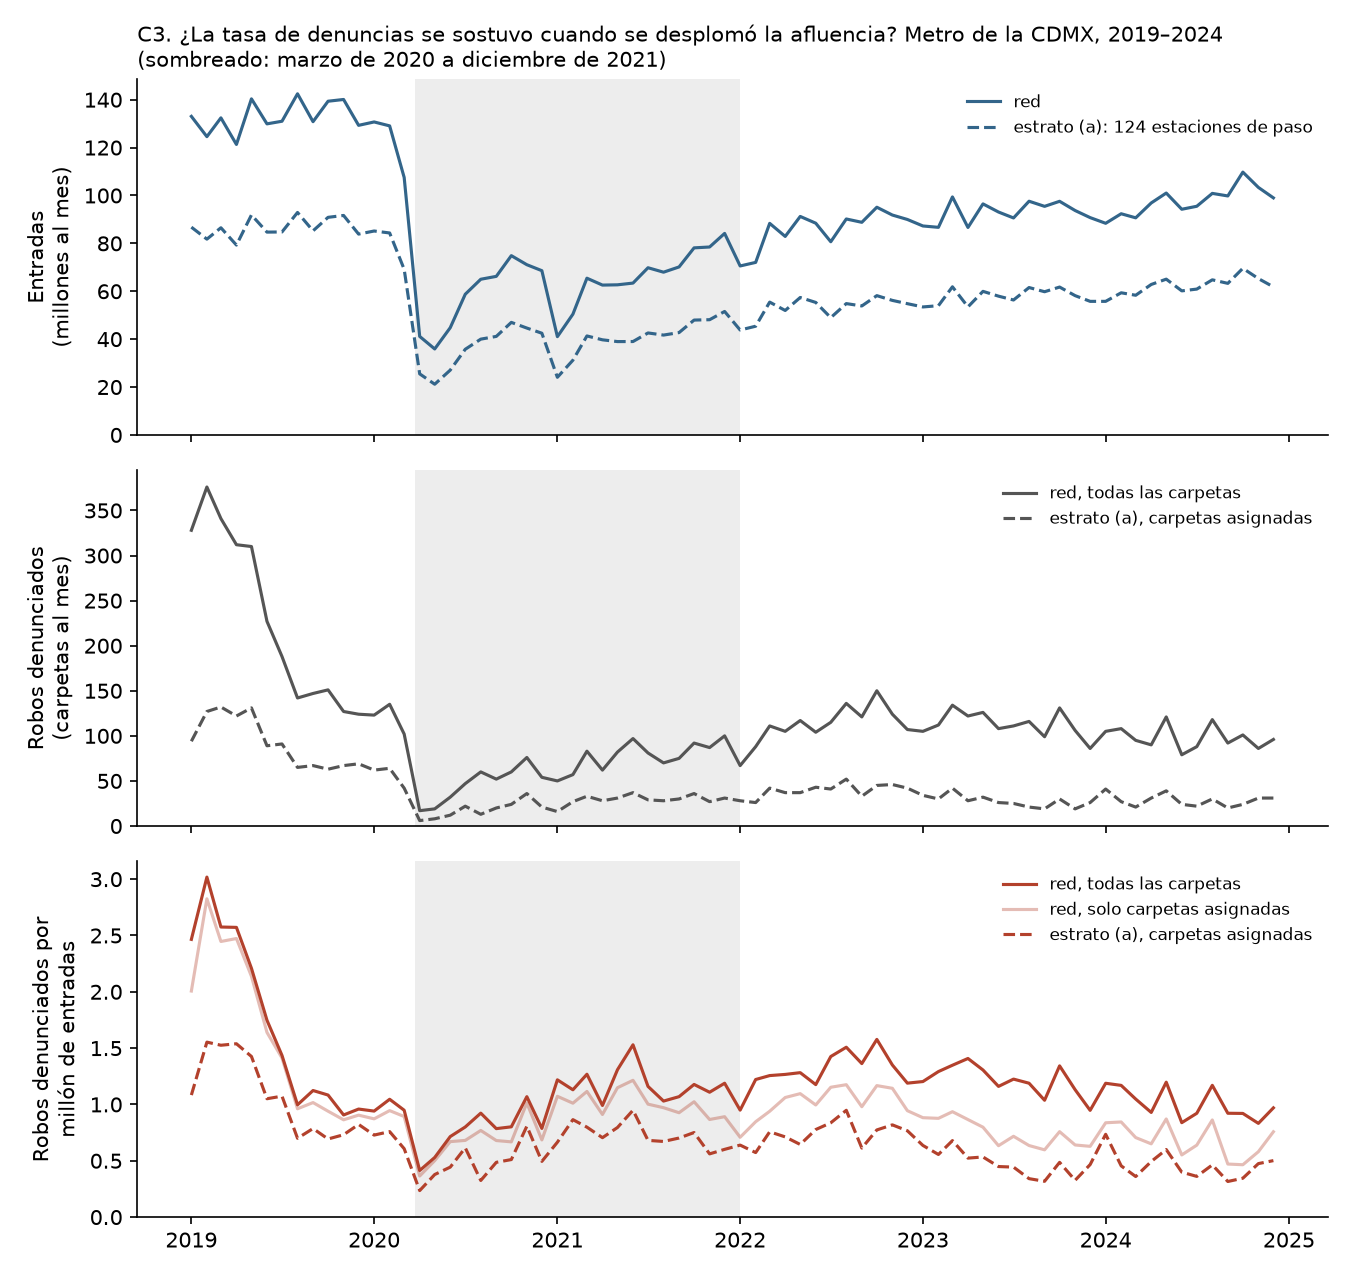
\includegraphics[width=0.85\columnwidth]{c3_tasa_vs_afluencia}
\caption{Tasa mensual de denuncias \pme{} y entradas en la red, 2019--2024. El quiebre grande de la serie ocurre dentro de 2019 con la afluencia plana; en el confinamiento la tasa cae a la mitad y después vuelve al nivel previo con la mitad de las entradas.}
\label{fig:c3}
\end{figure}

\subsection{Conteo contra tasa en las 124 estaciones de paso}

\textbf{T5.} En las 124 estaciones de paso (en adelante, el estrato: 2\,945 denuncias, 4\,170 millones de entradas, 0.71 \pme), la correlación de rangos entre el orden por conteo y el orden por tasa es $\rho = 0.454$ (intervalo al 95~\% por \emph{bootstrap}, es decir, con remuestreo de estaciones: 0.29 a 0.60) y solo 3 de las 10 primeras coinciden (fig.~\ref{fig:conteo_tasa}). El criterio de falla, fijado antes, era $\rho \geq 0.9$ y nueve coincidencias. El resultado no depende de las decisiones arbitrarias: con tres radios de asignación (100, 150 y 250~m) y tres mínimos de denuncias (0, 20 y 30), las nueve combinaciones dan $\rho$ de 0.097 a 0.457, y al exigir más señal la correlación baja. El desacuerdo no lo producen las estaciones chicas.

Lo que el conteo esconde son las terminales: Indios Verdes (114 denuncias, primera por conteo) queda en el lugar 73 por tasa, con 0.63 \pme; Constitución de 1917 pasa del 3 al 82 (0.55); Tasqueña, del 7 al 90 (0.52). Son estaciones con muchas denuncias y decenas de millones de entradas: los intervalos son estrechos y las tres están en la media del estrato o por debajo. Su tasa es ordinaria; lo que tienen es muchísima afluencia. Lo que sube es un grupo de estaciones medianas con tasa del doble del estrato que no aparece en ninguna lista publicada: Villa de Aragón, Nativitas, Portales y Merced (40 a 90 denuncias). Y hay movimientos que son ruido: Tlaltenco sube 109 lugares con 5 denuncias y un intervalo de 0.44 a 3.20 (fig.~\ref{fig:intervalos}).

\begin{figure}[t]
\centering
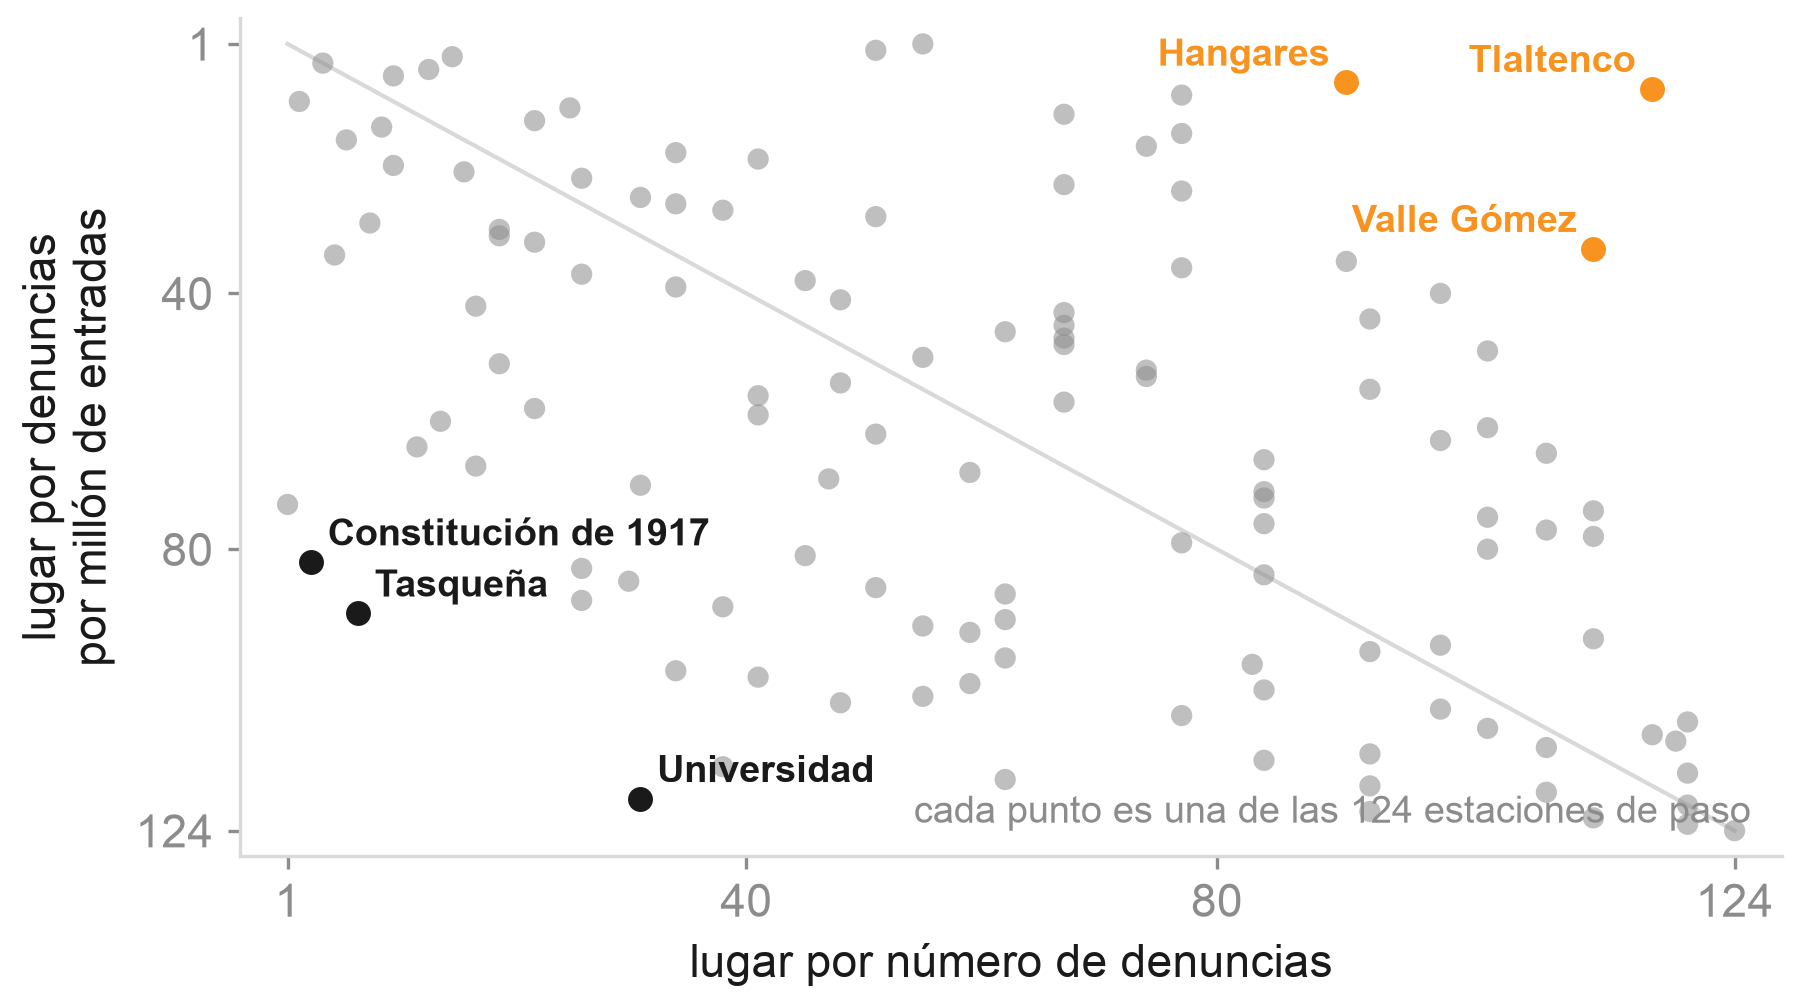
\includegraphics[width=\columnwidth]{conteo_vs_tasa}
\caption{Lugar por conteo contra lugar por tasa cruda, 124 estaciones de paso, 2019--2024. $\rho = 0.454$; 3 de 10 en común en la cabeza. Las terminales (negro) bajan; las que más suben (naranja) tienen entre 5 y 12 denuncias.}
\label{fig:conteo_tasa}
\end{figure}

\begin{figure}[t]
\centering
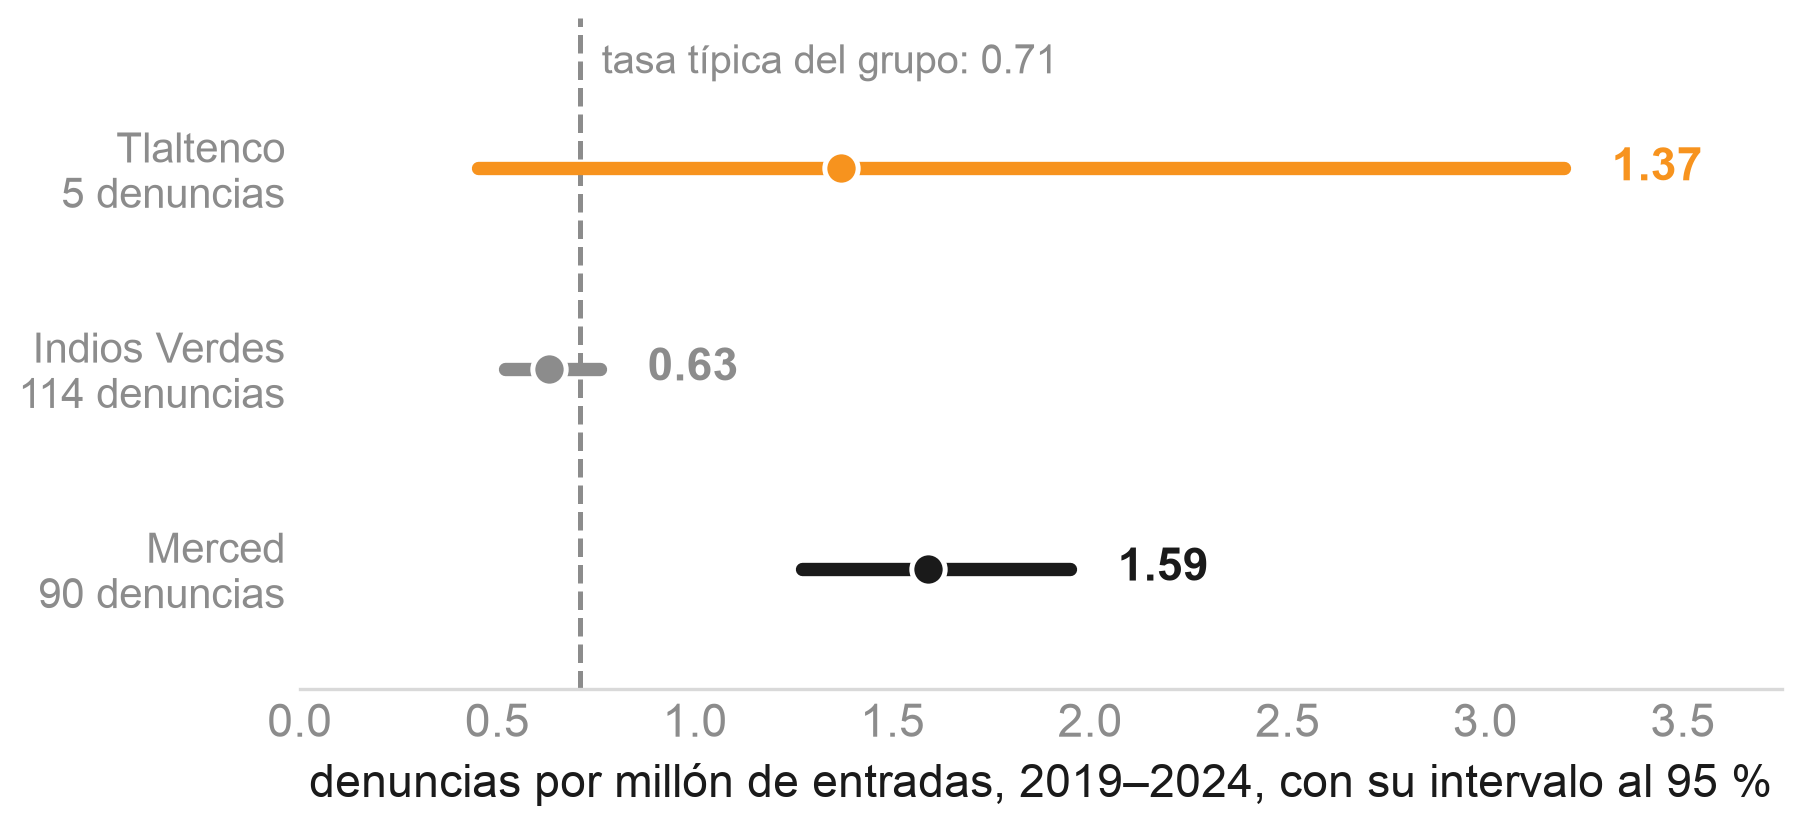
\includegraphics[width=\columnwidth]{intervalos}
\caption{Con pocas denuncias la tasa engaña: intervalos de Poisson al 95~\% \cite{ulm1990} de tres estaciones. Tlaltenco tiene la tasa más alta de las tres y su intervalo cubre la tasa típica; Indios Verdes, con 114 denuncias, se distingue por abajo.}
\label{fig:intervalos}
\end{figure}

\textbf{Análisis exploratorio (EDA) y lo que le pidió al modelo.} La estación mediana tiene 18 denuncias en seis años, tres al año; 42 de las 124 tienen menos de 15. La concentración es moderada (las diez primeras reúnen el 26.5~\% de las denuncias del estrato). Entre años la varianza es 2.3 veces la media (en un conteo de Poisson son iguales; el exceso se llama sobredispersión), pero entre meses, sin R1 ni R2, es 1.00: casi toda la sobredispersión aparente era el salto de 2019 y la heterogeneidad entre estaciones, así que la binomial negativa, un modelo de conteos que admite ese exceso, se probó y no se supuso. Con pruebas una por una al 95~\%, 39 estaciones se distinguen del estrato cuando por azar se esperarían unas seis; pero solo 19 de esas 39 siguen distinguiéndose al quitar cualquier año de los seis (las 19 robustas; las otras 20 son frágiles), y 36 de 39 con los tres radios. Cuatro de cada diez denuncias declaran un hecho entre las 6:00 y las 9:59 de la mañana; como la afluencia abierta es diaria y no horaria, ese perfil es de conteos y no de riesgo, y la hora no entra al modelo.

\subsection{El modelo}
\label{sec:modelo}

Sobre el panel estación por año del estrato (124 estaciones, hasta seis años, 715 celdas, 2\,919 denuncias sin abril--junio de 2020, 14.5~\% de celdas en cero):
\begin{gather}
y_{st} \sim \mathrm{NB}(\mu_{st}, \phi), \qquad v_s \sim N(0, \sigma_v^2), \nonumber \\
\log \mu_{st} = \log E_{st} + \alpha + v_s + \gamma_t,
\end{gather}
con $y_{st}$ las denuncias de la estación $s$ en el año $t$, NB la binomial negativa, $\phi$ su parámetro de sobredispersión (más chico, más varianza sobre la Poisson), $E_{st}$ los millones de entradas de la estación en los meses abiertos, $v_s$ el efecto de la estación, $\sigma_v$ cuánto difieren las estaciones entre sí, $\gamma_t$ el efecto de año con suma cero y $\exp(\alpha + v_s)$ la cantidad de interés: la tasa de la estación en un año promedio, encogida hacia la del estrato en proporción a la poca evidencia que tenga. Se ajustó por máxima verosimilitud marginal escrita a mano sobre \texttt{scipy}, con cuadratura de Gauss--Hermite adaptativa por estación \cite{liupierce1994}; la Poisson es el caso $\phi \to \infty$ del mismo código. Ninguna librería instalada ajustaba este modelo; son nueve parámetros y una integral por estación.

\textbf{Qué sale.} La binomial negativa gana a la Poisson (tabla~\ref{tab:modelos}, en el apéndice~C; razón de verosimilitudes LR $= 21.4$, $p < 10^{-4}$, corregida porque la Poisson está en la frontera, $\phi \to \infty$), pero la sobredispersión que queda es leve: $\phi = 16.5$ (intervalo de confianza al 95~\%, IC: 9.2 a 29.5) implica un 24~\% de varianza extra sobre la Poisson en una celda típica. Importa de todos modos: el orden casi no cambia ($\rho = 0.997$), pero la Poisson distinguiría 37 estaciones y la binomial negativa 25. La estación típica tiene $\exp(\alpha) = 0.633$ denuncias \pme{} (0.580 a 0.691); $\sigma_v = 0.402$ (0.333 a 0.486), de modo que el 95~\% de las estaciones cae entre 0.45 y 2.2 veces la típica. El efecto de año $\exp(\gamma_t)$ es 1.67 en 2019, 0.96, 1.11, 1.11, 0.73 y 0.70 en 2024: el 1.67 es el régimen R1, y la caída de 2023--2024 mezcla una baja real con las coordenadas que faltan.

\textbf{El encogimiento y la multiplicidad.} El orden encogido casi no cambia frente al crudo ($\rho = 0.985$); lo que cambia son los valores: Bosque de Aragón pasa de 2.08 a 1.40 \pme; Obrera, de 0.04 a 0.28. El factor de encogimiento (qué parte de su distancia a la estación típica conserva cada estación; 1 es no encoger) tiene mediana 0.60 con menos de 15 denuncias y 0.83 con 40 o más. Frente a una corrección por comparaciones múltiples (exigir más a cada prueba porque se hacen 124), que ensancha todos los intervalos por igual y trata igual a Merced (90 denuncias) que a Hangares (12), el modelo jerárquico estima de los datos cuánto varían de verdad las estaciones y jala a cada una hacia el centro en proporción a su evidencia \cite{gelman2012}. Quedan 25 estaciones distinguibles de la típica, es decir, con un intervalo al 95~\% que no incluye la tasa típica (14 por arriba, 11 por abajo), contra 39 de las pruebas una por una; el modelo conserva las 19 que el EDA había encontrado robustas y descarta 14 de las 20 frágiles, sin inventar ninguna nueva. Las 14 por arriba: Bosque de Aragón, Ciudad Deportiva, Villa de Aragón, Portales, Nativitas, Merced, Zócalo/Tenochtitlan, Etiopía, Camarones, Moctezuma, Insurgentes, Revolución, Niños Héroes y Polanco. Tasqueña, Indios Verdes y Constitución de 1917 no quedan como distinguibles por abajo (0.83, 1.01 y 0.88 veces la típica, con intervalos que incluyen 1): son terminales con tasa en la media.

\textbf{M3 se rechaza, y eso cambia el producto.} Hangares, con 12 denuncias, sigue en el lugar 10 por tasa encogida con un intervalo (0.90 a 2.52 veces la típica) que incluye 1. El encogimiento solo no protege de la poca evidencia: hay que ordenar por la tasa encogida y, además, mirar el intervalo. Por eso la aplicación marca como evidencia insuficiente todo lo que tenga menos de 15 denuncias: esa regla hace falta además del modelo.

\subsection{Fuera de muestra, y tres listas para desplegar}
\label{sec:listas}

Se ajustó el modelo con 2019--2023 y se midió contra 2024: 118 estaciones abiertas, 341 denuncias, mediana de 2 por estación y 20 estaciones en cero. El orden observado de 2024 es, en buena parte, ruido. La tasa predicha (la encogida del ajuste 2019--2023) correlaciona con la observada en 2024 con $\rho = 0.303$ (\emph{bootstrap}: 0.117 a 0.464), contra 0.261 de la tasa cruda y 0.289 del conteo. Si la tasa predicha fuera la verdad exacta, el $\rho$ contra un 2024 simulado con ruido de Poisson sería 0.376 en promedio: el modelo predice casi todo lo que se puede predecir de un año con 341 denuncias. Frente a la tasa cruda la mejora es consistente ($+0.042$, intervalo $+0.008$ a $+0.079$); frente al conteo no se distingue ($+0.014$, $-0.170$ a $+0.192$). M5 se sostiene por la letra y así se reporta.

\begin{table}[t]
\centering
\caption{Métrica de decisión, fuera de muestra: estaciones elegidas con 2019--2023 y lo que cubrieron en 2024 (341 denuncias y 747 millones de entradas en el estrato). $k$: estaciones elegidas. Prioridad: promedio del lugar por conteo y por tasa (§\ref{sec:listas}). Oráculo: la lista que se haría con el conteo real de 2024, como techo.}
\label{tab:cobertura}
\small\setlength\tabcolsep{3pt}
\begin{tabular}{@{}llrrr@{}}
\toprule
$k$ & Lista & Denuncias & Por millón & Entr. (M) \\
\midrule
10 & por conteo & \textbf{92} & 0.57 & 160 \\
10 & por tasa predicha & 41 & \textbf{0.77} & 53 \\
10 & prioridad & 59 & 0.75 & 79 \\
10 & \emph{oráculo (conteo de 2024)} & \emph{100} & \emph{0.70} & \emph{143} \\
\midrule
20 & por conteo & \textbf{135} & 0.58 & 233 \\
20 & por tasa predicha & 73 & 0.61 & 120 \\
20 & prioridad & 99 & \textbf{0.68} & 146 \\
20 & \emph{oráculo (conteo de 2024)} & \emph{163} & \emph{0.72} & \emph{227} \\
\bottomrule
\end{tabular}
\end{table}

\textbf{La métrica de decisión (M6).} A quien despliega le importa qué cubren las estaciones elegidas más que el orden entero (tabla~\ref{tab:cobertura}). Las diez elegidas por conteo cubren 92 denuncias de 2024, más del doble que las diez por tasa (41), y casi lo mismo que el oráculo que conociera el conteo real de 2024 (100): para cubrir volumen, el conteo es una regla excelente. Las diez por tasa predicha cubren 0.77 denuncias \pme{} contra 0.57, un 35~\% más por pasajero vigilado, con un tercio de la afluencia que vigilar (53 contra 160 millones de entradas), y superan a la tasa cruda en las dos métricas (28 denuncias y 0.69). Son dos objetivos distintos: cubrir volumen o igualar el riesgo por usuario. Hoy solo se publica la lista del primero, y sin declararlo.

\textbf{La lista de prioridad (volumen y riesgo).} Los sinodales pidieron, el 15 de octubre, una tercera lista que contemple las dos; en el registro de decisiones del repositorio aparece como lista combinada (decisión 65), y en la aplicación es el tercer botón, el de prioridad. Se evaluaron trece reglas fuera de muestra en dos años de prueba (2023 con ajuste 2019--2022, y 2024) con un criterio escrito antes de ver la tabla: cubrir al menos el 60~\% de lo que cubre el conteo con la mayor tasa, en $k = 10$ y 20 y en los dos años. Ninguna regla lo cumplió, porque la mejor cambia de año y de $k$, como corresponde a una señal débil de un año al siguiente. Se aplicó la regla de reserva que el criterio traía para ese caso, preferir la más simple de decir, entre las que superan al conteo en denuncias \pme{} y a la lista por tasa en denuncias cubiertas en los cuatro casos (esta exigencia se fijó después de ver la tabla): el promedio del lugar por conteo y del lugar por tasa encogida, solo entre estaciones con 15 denuncias o más. En 2024 sus veinte estaciones cubrieron 99 denuncias a 0.68 \pme: más tasa que la lista por tasa con un tercio más de denuncias, y 17~\% más tasa que el conteo con el 60~\% de la afluencia. En el \emph{bootstrap} sobre estaciones su ventaja sobre el conteo es positiva en el 99.4~\% de las remuestras en 2024 ($k = 20$) y en el 78~\% en 2023. Se recalcula a mano y no pierde frente a ninguna de las dos listas que ya existían, aunque no se afirma que sea la óptima.

\begin{figure*}[t]
\centering
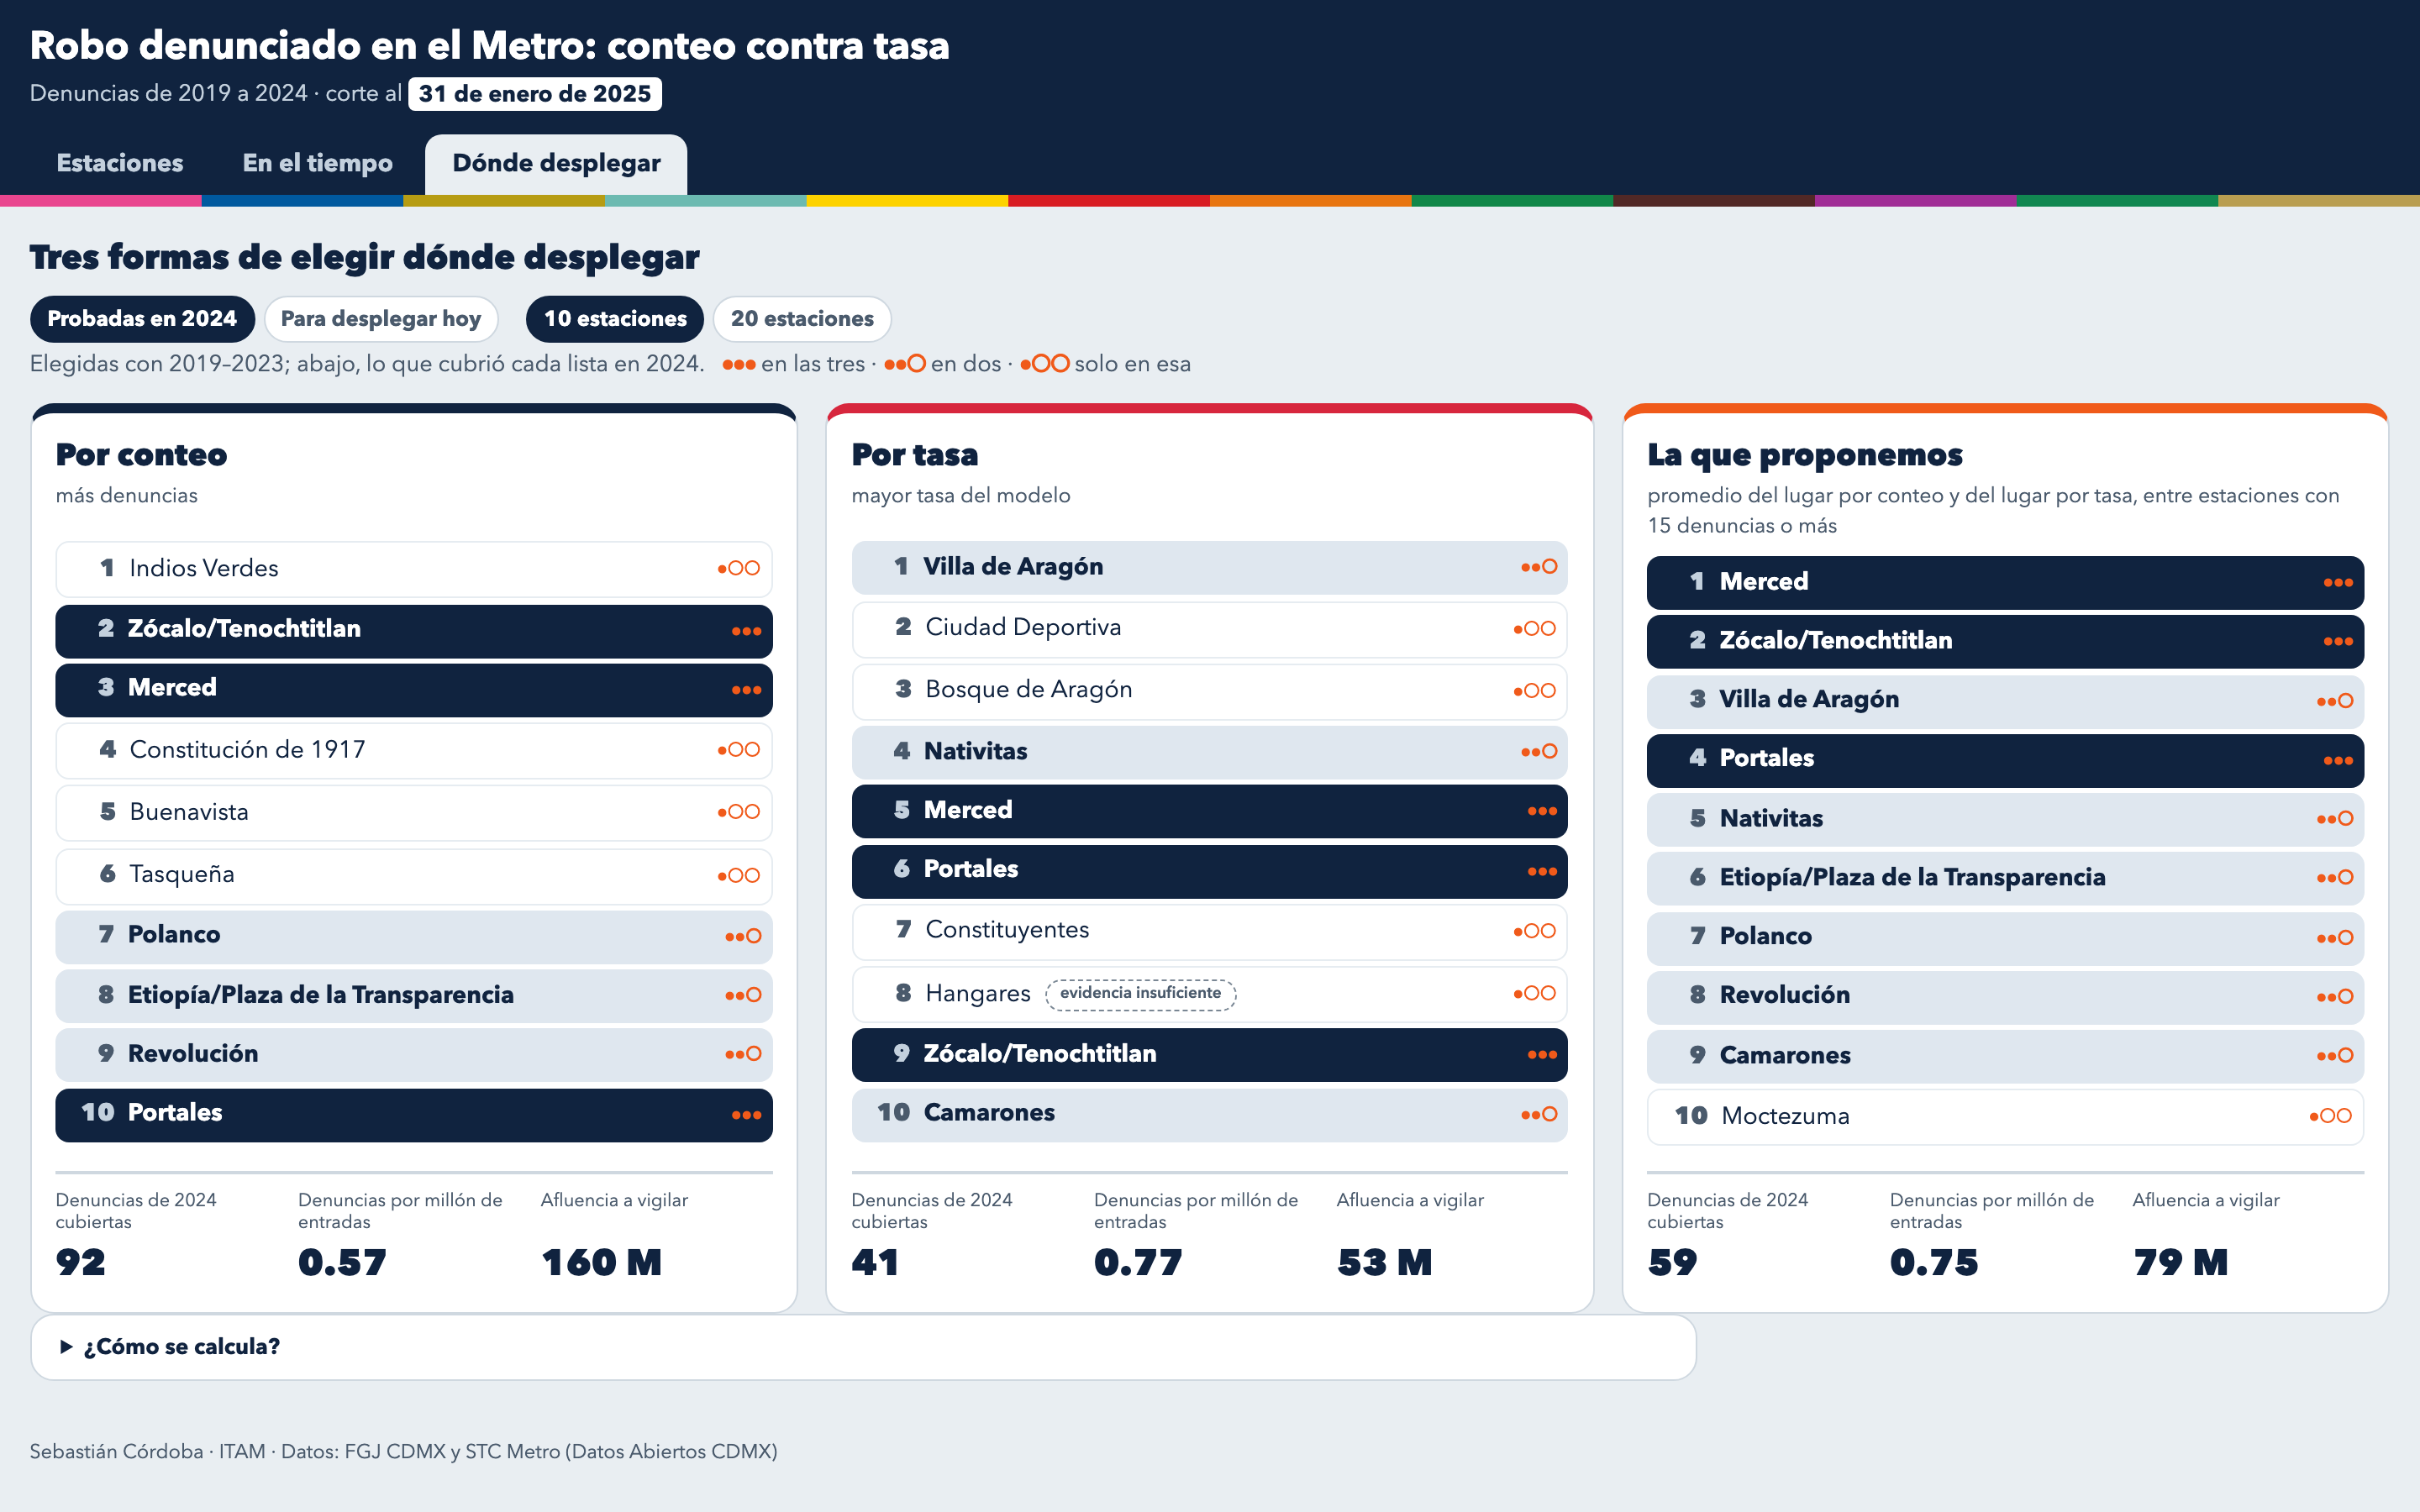
\includegraphics[width=0.72\textwidth]{app_captura_listas}
\caption{La aplicación, pestaña Dónde desplegar: las tres listas elegidas con 2019--2023 y lo que cubrió cada una en 2024. Los puntos indican en cuántas de las tres listas está cada estación. Captura del 24 de octubre de 2026.}
\label{fig:app}
\end{figure*}

\textbf{¿Más información predice mejor? No.} Con un protocolo escrito y registrado en git antes de correrlo, se añadieron al modelo covariables: características de cada estación calculadas solo con los años de entrenamiento. Son la línea, las carpetas de cualquier delito y de robo a transeúnte a 500~m de la estación (entorno), el tamaño y una tendencia propia de cada estación. Se evaluaron siete modelos en tres años de prueba rodantes (2022, 2023 y 2024) con la métrica de M6, el $\rho$ de M5 y un \emph{bootstrap} pareado, que remuestrea las mismas estaciones para los dos modelos (tabla~\ref{tab:covariables}, apéndice~C). Ningún modelo cumplió el criterio de mejora: en cada caso hay uno distinto que le gana al base por poco y pierde en los demás. Las covariables sí explican diferencias entre estaciones: con todas, $\sigma_v$ baja de 0.402 a 0.282, el 51~\% de la varianza en escala logarítmica; las estaciones grandes tienen un 20~\% menos denuncias por entrada y el robo a transeúnte alrededor va con un 12~\% más. Pero el modelo base ya aprende el nivel de cada estación de su propia historia, y lo que cambia de un año al siguiente es ruido de conteos pequeños. La tendencia extrapolada hace daño (0.56 contra 0.77 en 2024, $k = 10$). El límite lo pone el fenómeno medido con denuncias, y saber más de cada estación no lo mueve.


\subsection{La aplicación}

La aplicación \cite{app_metro} es una página estática, hecha con HTML, CSS y JavaScript propios y un solo archivo de datos de 170~KB. No usa servidor ni dependencias externas, funciona sin conexión y está diseñada para quien reparte elementos entre estaciones (fig.~\ref{fig:app}). Un selector de tres botones (conteo, tasa y prioridad, con el que abre) reordena la lista y el plano: Indios Verdes encabeza el conteo y, con un clic, queda en el lugar 67 por tasa encogida (73 por la cruda). El plano es esquemático con el centro ampliado, porque ahí está el interés y en una demostración nadie acerca nada; las correspondencias se dibujan chicas y con trama, para no fingir que son comparables; los tres estatus (por arriba, por abajo, no distinguible) se codifican con forma y no solo con color; y las estaciones con menos de 15 denuncias van marcadas como evidencia insuficiente y se dibujan huecas, de modo que Hangares (M3, la hipótesis rechazada) se ve tal como es. Una pestaña muestra la serie por año, y la pestaña Dónde desplegar, las tres listas (conteo, tasa y prioridad) lado a lado con lo que cubrió cada una en 2024, con la etiqueta de que fueron elegidas con 2019--2023, y la versión para desplegar hoy, con el ajuste completo. Los números escritos en la página se comprueban contra el modelo en cada regeneración.


\subsection{Herramientas y uso de IA generativa}

Python 3.13 con \texttt{pandas}, \texttt{geopandas} y \texttt{scipy}. El trabajo se hizo con asistencia de Claude Code (Anthropic), en diecisiete sesiones registradas una por una en el repositorio con lo que se pidió, lo que produjo y lo que se usó \cite{repo_caso}. La herramienta escribió el código del \emph{pipeline} (la cadena de programas de los datos a las tablas), del modelo y de la aplicación, propuso criterios de rechazo que quedaron escritos antes de correr, y redactó los documentos de cada fase. Las decisiones son del autor (el encuadre, los supuestos, qué se afirma y qué se descarta), y cada cifra de este escrito se recalculó sobre los archivos del repositorio antes de entrar. Lo que la herramienta no pudo abrir no se cita. Las correcciones a afirmaciones falsas se conservan tachadas en los documentos del repositorio, con fecha y causa.

\section{Conclusiones}

\textbf{La respuesta.} La lista pública de ``las estaciones más peligrosas'' ordena por número de denuncias, y ese orden es en buena parte un orden por afluencia. En las 124 estaciones de paso de la Ciudad de México, al dividir entre quién pasa el orden cambia: $\rho = 0.454$ entre las dos listas y 3 de las 10 primeras en común. Las grandes terminales (Indios Verdes, Constitución de 1917, Tasqueña) encabezan el conteo y son ordinarias por pasajero. Un grupo de estaciones medianas (Villa de Aragón, Nativitas, Portales, Merced, Bosque de Aragón, Ciudad Deportiva) tiene el doble de la tasa del estrato y no aparece en ninguna lista publicada. Las estaciones distinguibles de la típica son 25, no 39; las demás no se distinguen con estos datos. La diferencia es estable fuera de muestra: elegir con la tasa cubre más riesgo por pasajero con un tercio de la afluencia; elegir con el conteo cubre más del doble de denuncias.

\textbf{Recomendaciones, en orden de lo que cambia con menos esfuerzo.}
\begin{enumerate}
\item \emph{Publicar las tres listas y declarar el objetivo.} La autoridad publica una lista por conteo sin decir qué optimiza. Publicar al lado la lista por tasa y la de prioridad, con lo que cubre cada una, no cuesta datos nuevos: todo sale de los que ya son públicos, con un \emph{pipeline} que corre en minutos.
\item \emph{Usar la tasa, o la de prioridad, cuando el objetivo sea igualar el riesgo por pasajero.} Si el objetivo es cubrir volumen de denuncias, el conteo de los cinco años anteriores es una regla excelente y no hay que cambiarla. Si es que un pasajero tenga la misma protección en Nativitas que en Indios Verdes, sirve la de tasa, o la de prioridad si también importa el volumen (tabla~\ref{tab:cobertura}).
\item \emph{No mover recursos por estaciones con menos de 15 denuncias o cuyo intervalo toca la tasa típica.} El encogimiento no basta (M3); el intervalo es el filtro.
\item \emph{La franja de la mañana.} Cuatro de cada diez denuncias declaran un hecho entre las 6:00 y las 9:59, lo que dice cuándo se denuncia más, no cuándo es más probable por pasajero (no hay afluencia por hora); con esa advertencia, sirve para la franja del despliegue.
\end{enumerate}

\textbf{Implementación.} Viabilidad: tres fuentes abiertas, un repositorio público con el código y las decisiones, y una aplicación sin servidor que se regenera con un comando. Costo: cero en datos; horas de analista para actualizar cuando la FGJ publique un nuevo acumulado. Riesgos: las carpetas se corrigen después de publicadas, así que la lista debe llevar la fecha de corte (31 de enero de 2025) y el \emph{hash} del archivo; las coordenadas faltan cada vez más desde 2022, lo que sesga a la baja los años recientes; la prensa reporta caídas fuertes del robo en el metro en 2025 y 2026 que estos datos no ven. Y el riesgo de fondo: una tasa alta puede ser más robo o más disposición a denunciar. Se descartó el mecanismo más obvio, la agencia del Ministerio Público, pero no otros.

\textbf{Supuestos que, si cambian, cambian la recomendación.} Si el subregistro variara mucho entre estaciones de paso, el orden por tasa mediría dónde se denuncia y no dónde se roba. Si existiera una matriz de transbordos por estación, las 28 correspondencias entrarían al orden y la pregunta se extendería a toda la red. Si las carpetas sin coordenadas faltaran más en unas estaciones que en otras, el efecto de año no bastaría para absorberlo.

\textbf{Trabajo futuro.} Reconstruir la exposición de las correspondencias con la Encuesta Origen-Destino 2017 del INEGI y volver a probar C2. Pedir al STC la afluencia horaria para convertir el perfil de hora en riesgo. Explicar el exceso de Hidalgo y Guerrero y el quiebre de enero a agosto de 2019. Y cruzar, cuando exista, una medida de victimización por estación que diga cuánto de la tasa es denuncia y cuánto es robo.

\bibliographystyle{IEEEtran}
\bibliography{referencias}

\appendices

\section{Reproducibilidad}

Todo se regenera desde el repositorio \cite{repo_caso} con Python 3.13:
\begin{verbatim}
python src/descarga.py --fuente estaciones
python src/metro/correr.py
bash docs/escrito/compila.sh
\end{verbatim}
El primer comando baja las carpetas de la FGJ (534~MB), la afluencia y el \emph{shapefile}, y escribe su \emph{hash} en \texttt{datos/crudos/MANIFIESTO.md}. El segundo corre en orden la llave de estaciones, el panel, las pruebas C1--C3, las agencias, T5, el EDA, el modelo, las tres listas, las covariables y, al final, los datos de la aplicación, que se arman con lo anterior; cada paso contiene sus comprobaciones (\texttt{assert}) y se detiene si una falla o si una prueba manda parar. Las figuras de este escrito salen de esos scripts; el escrito se compila con \texttt{tectonic}. Las 71 decisiones, con fecha, alternativa descartada y razón, están en \texttt{docs/decisiones.md}; las hipótesis congeladas, en \texttt{docs/hipotesis.md}.

\section{Registro de uso de IA generativa}

El registro completo está en \texttt{docs/uso-ia.md} del repositorio: una fila por sesión, con fecha, herramienta, qué se pidió, qué produjo y qué se usó. Resumen de las diecisiete sesiones (20 de septiembre a 26 de octubre de 2026), todas con Claude Code: exploración de factibilidad de cinco encuadres y elección del metro; llave de estaciones, panel y pruebas C1--C2; agencias del Ministerio Público (T0--T7) y registro de las listas publicadas; compuerta T5 y C3; aplicación estática y su publicación; hipótesis congeladas, EDA y modelo; dos actualizaciones de la aplicación; dos presentaciones ante los sinodales y sus guiones; la tercera lista; el protocolo de covariables y su resultado negativo; y este escrito. En cada fila se distingue lo que fue iniciativa de la herramienta de lo que pidió el autor, y se anotan los errores que la herramienta cometió y cómo se detectaron, entre ellos un ajuste que resultó Poisson por una cadena en mayúsculas y una lista de prensa mal atribuida en un borrador de presentación.

% Las dos tablas van juntas arriba de una página nueva, a todo lo ancho, debajo del título
% del apéndice: como flotantes de una columna caían solas en la última página.
\twocolumn[{%
\section{Dos tablas del modelo}
\begin{center}
\begin{minipage}{0.86\textwidth}
\small Estas dos tablas completan las secciones~\ref{sec:modelo} y~\ref{sec:listas}: la tabla~\ref{tab:modelos} compara los cuatro modelos ajustados, y la tabla~\ref{tab:covariables} resume la prueba de covariables, cuyo detalle por año, $k$ y modelo está en \texttt{docs/covariables.md}.
\end{minipage}

\vspace{1.2em}
\begin{minipage}{0.62\textwidth}
\centering
\captionof{table}{Poisson contra binomial negativa (NB), con y sin efecto de estación. Todas con efecto de año. $k$: número de parámetros; log-ver.: log-verosimilitud; AIC: criterio de Akaike, menor es mejor.}
\label{tab:modelos}
\small\setlength\tabcolsep{4pt}
\begin{tabular}{@{}lrrrrr@{}}
\toprule
Modelo & $k$ & log-ver. & AIC & $\sigma_v$ & $\phi$ \\
\midrule
Poisson, sin efecto de estación & 6 & $-1\,649.8$ & 3\,311.6 & --- & --- \\
NB, sin efecto de estación & 7 & $-1\,527.8$ & 3\,069.7 & --- & 4.5 \\
Poisson + efecto de estación & 7 & $-1\,492.9$ & 2\,999.8 & 0.427 & --- \\
\textbf{NB + efecto de estación} & 8 & $\mathbf{-1\,482.2}$ & \textbf{2\,980.3} & 0.402 & 16.5 \\
\bottomrule
\end{tabular}
\end{minipage}

\vspace{1.6em}
\begin{minipage}{0.86\textwidth}
\centering
\captionof{table}{Más información no mejora la predicción: modelo base contra el mejor de seis modelos con covariables, por métrica, con el criterio fijado antes de correr. Techo: el $\rho$ que se obtendría si la tasa predicha fuera la verdadera, por el solo ruido de conteo de un año. Casos: tres años de prueba por dos tamaños de lista ($k = 10$ y 20). Todas las fijas: línea, entorno y tamaño.}
\label{tab:covariables}
\small\setlength\tabcolsep{5pt}
\begin{tabular}{@{}lrrl@{}}
\toprule
Métrica & Base & Mejor nuevo & Cuál \\
\midrule
$\rho$ entre tasa predicha y observada, 2024 & 0.303 & 0.324 & entorno \\
Techo por ruido de ese $\rho$ & 0.376 & --- & --- \\
Top-10 por tasa, 2024, denuncias \pme & 0.773 & 0.799 & línea \\
Top-20 por tasa, 2024, denuncias \pme & 0.610 & 0.658 & entorno \\
Top-10 por tasa, 2022, denuncias \pme & 1.220 & 1.150 & entorno \\
Modelos que ganan en $\geq 4$ de los 6 casos & --- & ninguno & --- \\
$\sigma_v$ en el ajuste completo & 0.402 & 0.282 & todas las fijas \\
\bottomrule
\end{tabular}
\end{minipage}
\end{center}
\vspace{1em}
}]

\section{Las 124 estaciones}

El lugar de cada una de las 124 estaciones en las tres listas, con sus denuncias, entradas, tasa encogida e intervalo, está en \texttt{datos/procesados/metro\_tablas/tres\_listas.csv}, se regenera con el \emph{pipeline} del apéndice A y se consulta en la aplicación \cite{app_metro}. Las veinte primeras por tasa encogida, con intervalo, están en \texttt{docs/modelo.md}.

\end{document}
